% **************************************************************************** %
%                                                                              %
%                                                         :::      ::::::::    %
%    sec_mteorico.tex                                   :+:      :+:    :+:    %
%                                                     +:+ +:+         +:+      %
%    By: acampo-p <acampo-p@student.42urduliz.com>  +#+  +:+       +#+         %
%                                                 +#+#+#+#+#+   +#+            %
%    Created: 2022/12/07 17:42:28 by acampo-p          #+#    #+#              %
%    Updated: 2023/02/13 04:11:09 by acampo-p         ###   ########.fr        %
%                                                                              %
% **************************************************************************** %

\section{MARCO TEÓRICO}

\subsection{SIMULACIÓN DE EVENTOS DISCRETOS}

Con el avance tecnológico experimentado desde los inicios de la computación,
nuevas maneras para afrontar la resolución de problemas han surgido,
que un siglo antes, habrían sido descartadas por su falta de viabilidad.
La capacidad de calculo y el diseño de inteligencias artificiales,
a proporcionado las herramientas necesarias
para solucionar aquellos problemas, que con métodos clásicos,
definitivamente demasiado complejos para modelar.
La simulación, hoy en día, es una de las tres metodologías consolidadas,
en el ámbito científico e ingenieril,
para la resolución de problemas \citep{banks1998handbook}.
Siendo esta metodología descrita como ``la técnica del ultimo recurso'',
por \citep{garzia1986discrete},
debido a la intensa demanda computacional
que requería en el momento de su publicación,
el transcurso de los años ha mermado esta desventaja.

Diversos autores describen la simulación de la siguiente manera

\begin{itemize}
	\item ``Una simulación es
	el establecimiento de un modelo lógico-matemático de un sistema
	y la manipulación experimental de este en una computadora digital
	\citep{pritsker1974gasp}''.   
	\item ``La simulación es el proceso de diseñar
		el modelo de un sistema real y realizar experimentos
		con este modelo con el propósito de,
		entender el comportamiento del sistema,
		o evaluar distintas estrategias
		(dentro de los limites impuestos por un criterio
		o conjunto de criterios)
		para la operación del sistema'' \citep{shannon1976systems}.
	\item ``Una simulación es la imitación de el modo de operación
		de un proceso real o sistema durante el transcurso del tiempo''
		\citep{banks1999introduction}.
\end{itemize}

Como se puede observar, el modelo,
es un termino recurrente en el ámbito de la simulación.
Banks sostiene que el modelo es la representación del sistema simulado
\citep{banks1998handbook}.
El autor matiza que la virtud de un modelo radica en su complejidad,
siendo necesario el balance entre una representación ajustada,
sin complicar en exceso el modelo.
Por tanto, aquellos factores que no influyan lo suficiente
en los resultados de la simulación, deberían ser eliminados,
ya que únicamente extienden el proceso de desarrollo.

El modelo, por tanto, constituye la base de la simulación,
define las variables, y criterios para las decisiones tomadas en la simulación.
Banks señala, la distinción entre un modelo matemático convencional
y el modelo de una simulación \citep{banks1998handbook}.
Los modelos matemáticos y estadísticos
suelen representar las variables de manera explicita,
relacionando variables independientes y variables dependientes
para obtener un resultado.
En el caso de una DES, el modelo utilizado se enfoca en
la representación de sus componentes internos y sus interacciones.

El funcionamiento de la DES, se basa en registrar los cambios
que van ocurriendo en el estado del sistema durante el transcurso del tiempo.
En el intervalo entre alternaciones de estado,
ocurren el concepto de eventos, propios de esta rama de simulación.
Varga \citep{varga2001discrete} describe estos eventos como instantáneos,
siendo la duración de los mismos nula.
Durante el evento no ocurre nada especial,
salvo la alteración del estado del sistema.
Una sencilla representación de este concepto
puede ser observada el la Figura~\ref{fig:2_fc_simple_ex},
donde el sistema representado es un coche.
El coche posee 3 estados, los cuales se van sucediendo,
durante el transcurso del tiempo.

\begin{figure}[h]
	\begin{center}
		\includestandalone{fig/2_fc_simple_ex}
	\end{center}
	\caption{Representación del cambio de estado en una DES,
	los rectángulos representan el estado del sistema,
	mientras que las flechas indican el suceso de un evento instantáneo.}
	\label{fig:2_fc_simple_ex}
\end{figure}

\subsubsection{Terminología y funcionamiento de una DES}\label{TF_DES}

Para describir detalladamente este tipo de simulaciones,
es necesario definir previamente algunos conceptos.
Los siguientes conceptos
son la síntesis de la información redactada por \citep{banks1998handbook}
aplicados en el entorno de Python y su librería Simpy.

\paragraph{Las variables del estado}
del sistema proporcionan información
acerca de el comportamiento de los procesos
que se llevan a cabo durante la simulación.
Determina las variables de estado que el programa debe retornar
depende de el objetivo del proyecto.
El programa deberá ser diseñado entorno a ellas,
puesto que,serán usadas
para el posterior calculo de indicadores del rendimiento.
Un ejemplo, es el momento de inicio y fin de un subproceso.

\paragraph{Las entidades}
son los objetos representados por el modelo.
Se distinguen dos tipos de entidades,
las dinámicas y las estáticas.
Las primeras, avanzan en el sistema
a través de los procesos simulados, 
mientras que las segundas, dan servicio a las primeras
permaneciendo ocupadas en el proceso.
Considerando una gasolinera como sistema,
la entidad dinámica seria un coche repostando combustible,
mientras que la estática, seria la estación de repostaje.
Estos objetos pueden poseer atributos,
como el consumo de combustible o el tamaño de su deposito.
Dependiendo de el objetivo de la simulación,
algunos atributos serán relevantes en diseño del modelo.

\paragraph{Un recurso}
es una entidad
que provee de servicio a una entidad dinámica.
Los recursos pueden servir a múltiples entidades simultáneamente.
De manera similar, una entidad puede
solicitar varios tipos de recursos en distintas cantidades.
Si la demanda de una entidad no se satisface,
esta entrara en una cola,
a la espera de la liberación del recurso.
Cuando la entidad tome el recurso,
lo mantendrá ocupado durante la duración del proceso.
Los recursos pueden tener varios estados,
como disponible, ocupado, averiado, en mantenimiento\ldots
Un ejemplo de recurso, puede ser el número de
estaciones de autoservicio que posee una gasolinera.

\paragraph{Una actividad}
es un periodo de tiempo,
el cual es conocido previo a su inicio.
Su duración puede ser determinada de varias maneras;
mediante una constante, una distribución estadística,
el resultado de una ecuación, un archivo o una decisión lógica.
El conocimiento de su duración,
supone saber cuando un recurso sera liberado,
lo que facilita el trabajo de computación.

\paragraph{Una demora}
es un periodo de espera indefinido
antes del comienzo de una actividad.
Este depende de la ejecución
de el resto de actividades prioritarias,
por lo que el final de la espera no se puede determinar
mientras el recurso siga ocupado.

\paragraph{Un evento}
ocurre al principio y al final de una actividad o demora.
Marcan la transición de el sistema de un estado a otro.

Considerando todos estos conceptos,
las entidades del sistema compiten entre ellas por el uso de los recursos,
si estos no se encuentran disponibles, quedan a la espera de poder solicitarlos.
Tanto las actividades como las demoras reclaman estas entidades
durante los intervalos entre eventos,
siendo liberadas para el siguiente proceso una vez finalizado el periodo.
Una DES, puede describirse como el avance de una entidad o conjunto de entidades
a través  de las actividades que modelan el proceso real.
Este avance es accionado
mediante el transcurso de tiempo virtual dentro de la simulación.

\subsubsection{Exposición de un caso ficticio usando una DES}\label{example_descrp}

Con el objetivo de ilustrar los conceptos descritos en la sección~\ref{TF_DES}
y demostrar la capacidad de resolución de problemas de la DES,
se ha procedido a emular un caso práctico.

Supóngase que un ayuntamiento ficticio desea disminuir
los problemas causados por el congestionamiento del trafico en la ciudad.
El ayuntamiento solicita a una consultoría ingenieril
desarrollar un proyecto para observar el
desempeño de las distintas soluciones planteadas.
La consultoría ve apropiado usar una DES para valorar
el impacto de las distintas propuestas
y proponer un plan de acción optimo a la entidad contratante.

El objetivo principal de el ayuntamiento es
minimizar la cantidad de vehículos que circulan por la ciudad.
Una de las causas de congestión apunta a una estación de repostaje
con unos precios particularmente competitivos
que causa complicaciones a la entrada de la ciudad.
Se cree que su capacidad de abastecimiento
no es suficiente durante los picos de alta actividad.
Por otra parte, la ciudad es un potente centro de actividad comercial.
Muchos empleados se desplazan a diario en coche,
lo que sumado a los espacios limitados de estacionamiento,
y la alta densidad poblacional,
hace sospechar que los conductores se demoran en exceso a la hora de buscar parking.
Se teme que este tiempo adicional,
sea un factor considerable en las emisiones totales de los vehículos.

Con las siguientes dos medidas se espera obtener
una reducción del congestionamiento del trafico en la ciudad.

\begin{itemize}
	\item Primeramente, negociar un ampliamiento
		del servicio de distribución de combustibles
		con la empresa propietaria de la estación de repostaje.
	\item Paralelamente, ampliar la capacidad de un parking publico gratuito
		ubicado cerca del núcleo de actividad laboral.
\end{itemize}

La simulación planteada, tratara de emular el comportamiento de los vehículos
que circulan por la ciudad durante el transcurso de una jornada laboral normal.
Es por ello que el comienzo de la simulación se estima entorno a las 7:00 a.m.
y se prologa hasta 9:00 p.m.
El modelo producirá 2 tipos de entidades,
el vehículo de tipo `A', que sera el medio de transporte para los trabajadores de la zona,
y el de tipo `B' que englobará todo tipo de usuarios ajenos a el ámbito laboral.
Esta distinción se ha considerado necesaria,
debido a la uniformidad que representa el primer grupo, respecto al segundo, algo más caótico.
Los vehículos generados seguirán la rutina descrita el la Figura~\ref{fig:2_fc_complex_ex}.

\begin{figure}
	\begin{center}
		\includestandalone{fig/2_fc_complex_ex}
	\end{center}
	\caption{Modelo del caso practico descrito en el apartado~\ref{example_descrp}}
		\label{fig:2_fc_complex_ex}
\end{figure}

La consultoría, por una parte, establece
las propiedades generales de su modelo en la Tabla~\ref{tab:2_tbl_spec01_ex}.
Mientras que, por otra parte, decide recopilar información clave
para el desarrollo del modelo de simulación.
A raíz de un análisis obtiene los datos mostrados en la Tabla~\ref{tab:2_tbl_spec02_ex}.

\begin{table}
	\centering
	\caption{Especificaciones generales.}
	\documentclass[varwidth=\maxdimen]{standalone}
\usepackage[utf8]{inputenc}
\usepackage[spanish]{babel}
\usepackage{booktabs}

\begin{document}

\begin{tabular}{ l c }
	\toprule
	Nombre	& Valor	\\
	\midrule
	Duración				& 960	min \\
	Ejecuciones				& 20	uds. \\
	Capacidad del parking	& 100	uds. \\
	Estaciones de repostaje	& 4		uds. \\
	Probabilidad de repostaje		& 50\% \\
	\bottomrule
\end{tabular}

\end{document}

	\label{tab:2_tbl_spec01_ex}
\end{table}
	
\begin{table}
	\centering
	\caption{Propiedades de las distribuciones observadas en las procesos reales.}
	\documentclass[varwidth=\maxdimen]{standalone}
\usepackage[utf8]{inputenc}
\usepackage[spanish]{babel}
\usepackage{booktabs}

\begin{document}

\begin{tabular}{ l c c c }
	\toprule
	Variable	& Tipo de vehículo	& Distribución	& Constantes (min) \\
	\midrule
	Conducir largo	& A y B	& Gamma			& $k = 8$, $\theta = 3$ \\
	Conducir corto	& A y B	& Triangular	& $min = 2$, $moda = 3$, $max = 4$ \\
	Buscar \textit{parking}	& A y B	& Gamma			& $k = 10$, $\theta = 1$ \\
	Repostar		& A y B	& Triangular	& $min = 4$, $moda = 5$, $max = 8$ \\
	Entre llegadas	& A*	& Exponencial	& $\lambda = 1$ \\
					& B		& Exponencial	& $\lambda = 15$ \\
	Estacionamiento	& A		& Normal		& $\mu = 560$, $\sigma = 60$ \\
					& B		& Lognormal		& $\mu = 5$, $\sigma = 0.7$ \\
	\bottomrule
\end{tabular}

\end{document}

	\footnotesize{*La generación de entidades tipo `A' únicamente se prolonga desde el comienzo de la simulación hasta el minuto X.
	Así, se obtiene una aproximación, a el horario típico de un día laboral.}
	\label{tab:2_tbl_spec02_ex}
\end{table}

Como puede observarse en la Figura~\ref{fig:2_fig_example_01},
la adición de 2 estaciones de autoservicio en la gasolinera
evita su colapso en intervalos críticos.
En el gráfico situado a la izquierda,
el pico de actividad azul entorno al minuto 150 de la ejecución de la simulación,
se ve drásticamente reducido, mientras que el repunte secundario es completamente eliminado.
A su vez, en el gráfico adyacente,
La desviación estándar de tiempos de espera queda reducida
y su media queda desplazada hacia el eje.

\begin{figure}
	\begin{center}
		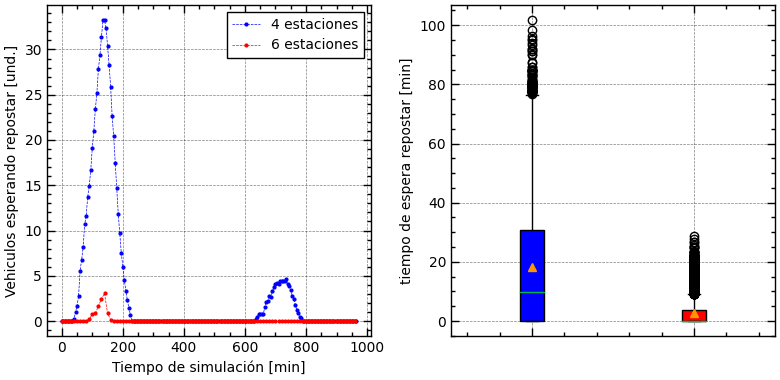
\includegraphics[width=\textwidth]{fig/2_fig_example_01}
	\end{center}
	\caption{Izquierda: Evolución de los vehículos a la espera de repostar para distintos escenarios. Derecha: Distribución de los tiempos de espera de repostaje para los distintos escenarios}
	\label{fig:2_fig_example_01}
\end{figure}

Continuando con el análisis, el la Figura~\ref{fig:2_fig_example_02},
El efecto de incrementar en un 50\% las plazas de parking disponible,
no es apreciable en el gráfico expuesto arriba.
La cantidad de vehículos en carretera permanece similar,
mientras que en el gráfico inferior los vehículos saturan el parking hasta su nuevo limite.
Al no haber una clara correlación entre ambos indicadores,
se ilustra la representación de la distribución de tiempos de conducción
en la Figura~\ref{fig:2_fig_example_03}.
En esta exposición, puede llegar a apreciarse una ligera diferencia en los tiempos de conducción,
aunque un test de hipótesis sería necesario
para determinar si estas diferencias son estadísticamente significativas.

En conclusión, los resultados muestran una clara ruta de inversión
a la hora de ampliar la estación de combustibles,
mientras que la expansión de el parking parece irrelevante.
Esto demuestra la capacidad de recopilación de datos que ofrece una DES.
Simultáneamente subraya la importancia del tratamiento de los datos obtenidos,
y el uso de pruebas estadísticas, para la obtención de conclusiones certeras.

\begin{figure}
	\begin{center}
		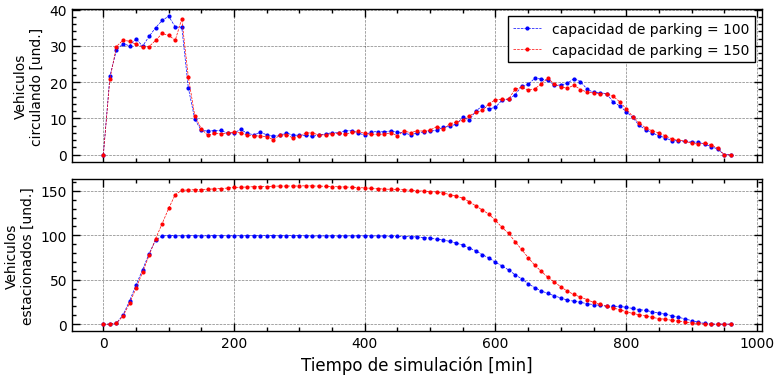
\includegraphics[width=\textwidth]{fig/2_fig_example_02}
	\end{center}
	\caption{Evolución de la cantidad de vehículos a lo largo de la simulación, en distintos escenarios. Arriba: Vehículos en circulación. Abajo: Vehículos estacionados.}
	\label{fig:2_fig_example_02}
\end{figure}

\begin{figure}
	\begin{center}
		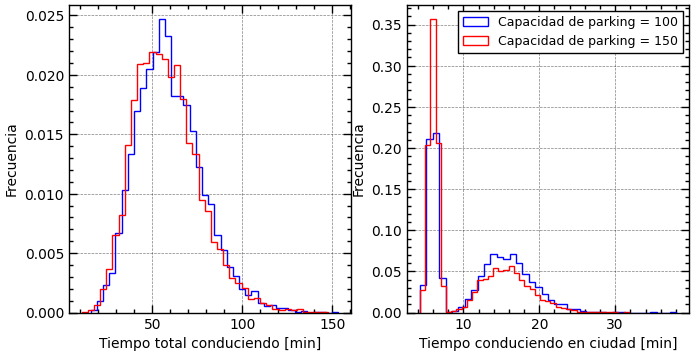
\includegraphics[width=\textwidth]{fig/2_fig_example_03}
	\end{center}
	\caption{Distribución de el tiempo de conducción para distintos escenarios. Izquierda: Tiempo total en circulación. Derecha: Tiempo circulando dentro de la ciudad.}
	\label{fig:2_fig_example_03}
\end{figure}

\subsubsection{Etapas de desarrollo de una DES}

Para que un proyecto tan complejo como una DES prospere, es fundamental estructurarlo.
El diagrama expuesto en la Figura~\ref{fig:2_fc_sim_cookbook} publicado por \citep{banks1998handbook}
define las etapas que deberían seguir este tipo de proyectos.
Al ser este proyecto un simple Trabajo de Fin de Grado,
este esquema servirá como orientación, más que como plano para la construcción de la simulación.
Por ejemplo, la recopilación de datos ha resultado imposible en el momento de redacción del trabajo,
pero se espera desarrollar el proyecto
a partir de las más ajustadas distribuciones de probabilidad supuestas para el desarrollo del modelo.
Se espera que este trabajo asiente una base,
y que las imperfecciones actuales puedan ser corregidas en el futuro.

\begin{figure}
	\begin{center}
		\includestandalone{fig/2_fc_sim_cookbook}
	\end{center}
	\caption{Esquema del proceso de desarrollo de una DES.}
	\label{fig:2_fc_sim_cookbook}
\end{figure}

\paragraph{Formulación del problema, establecimiento de objetivos, y plan general.}

Cada DES comienza con la declaración del problema que se tratará de solucionar.
Esta etapa es crucial debido a que el resto de el trabajo se asentara sobre esta base.
Se debe asegurar que el problema que se esta formulando sea el correcto,
la comunicación entre el cliente y el equipo desarrollador debe ser optima.
Una descripción precisa y un conocimiento extenso del sistema son necesarios para evitar
trabajar en solucionar el problema equivocado.
Es por ello que debe haber comunicación y feedback constante entre cliente y equipo.

En el caso de este trabajo, algo similar sucede.
Al ser un único autor, la comunicación no sera un factor importante,
pero esto conllevara otras complicaciones.
El autor debe, comprender profundamente el sistema a modelar, y a su vez,
dominar el uso de las herramientas de simulación.
Manejar ambas, requerirá recordar la formulación del problema inicial
más frecuentemente para no desviarse de la dirección.

Respecto a los objetivos, estos deben ayudar a asentar la dirección de trabajo actuando como plan general.
El establecimiento de varios objetivos alcanzables, cohesivos y correctamente secuenciados,
guiará el proceso de desarrollo.
Esto objetivos quedan listados en la sección~\ref{sec_obj}.

\paragraph{Conceptualización del modelo.}\label{sec:modelconcept}

El sistema propuesto sugiere conceptualizar el modelo en orden inverso,
es decir, comenzar identificando los objetivos del proyecto,
tal y como se ve en la Figura~\ref{fig:2_fc_model_concept}.

\begin{figure}[h]
	\begin{center}
		\includestandalone{fig/2_fc_model_concept}
	\end{center}
	\caption{Diagrama de pasos a seguir en la conceptualización de un modelo.}
	\label{fig:2_fc_model_concept}
\end{figure}

El siguiente paso es hallar las preguntas clave a las que
se les quiere dar respuesta.
Generar una lista, y ordenar las preguntas respecto a su relevancia es lo ideal.
Ademas, cuantificar los beneficios asociados a estas, aclara su jerarquía.

Después, se debe determinar que outputs son necesarios
para contestar a las preguntas previamente formuladas.
Introduciendo en la simulación únicamente la complejidad necesaria,
agilizará el proceso de desarrollo y mantendrá el enfoque original.

Continuando con el alcance de la simulación,
se deben detallar los procesos críticos en el calculo del \textit{output},
descartando o simplificando aquellos que no tengan gran impacto en la salida.
Por ejemplo, modelar recursos abundantes en la simulación,
no tendrá impacto en el output,
mientras que conocer los tiempos de espera de un proceso si lo hará.

Se Finaliza, especificando las variables independientes
que se introducirán al sistema.
Estas variables tienen que ser de alta calidad, ya que,
de lo contrario su introducción puede perjudicar al sistema al completo.
Un ejemplo seria el de distinguir entre distintas distribuciones
para entidades con atributos pobremente caracterizados.

\paragraph{Recopilación de datos.}

Cualquier DES requiere datos. La recopilación de la información del sistema,
o la estimación en caso de ser un sistema ficticio, es una necesidad.

\paragraph{Traducción del modelo.}

El modelo de simulación se construye a partir de la información desarrollada en el anterior punto.
Este proceso consiste en traducir de manera eficaz el esqueleto previamente desarrollado,
a un lenguaje que el ordenador pueda procesar.
Para ello Banks sugiere lo siguiente:

\begin{itemize}
	\item Enfoque en el problema. El proyecto no debería limitarse a desarrollar el modelo,
		si no que debería tratar de invertir aproximadamente el mismo tiempo
		en la exploración del sistema y la solución de problemas.
	\item Comienzo simple. El comienzo del proyecto debe ser simple,
		adquiriendo complejidad hasta alcanzar el detalle necesario.
	\item Manejo de la inteligencia del modelo.
		El modelo no debe superar el rendimiento de los procesos reales.
		El modelo desarrollado puede desarrollar ventajas respecto a su contrapartida real,
		como conocer la ubicación exacta de una pieza instantáneamente.
		Los humanos que gestionan el proceso difícilmente van a poder lograr este control,
		y supondrá una característica inalcanzable en el sistema real.
	\item Revisión. Revisar el funcionamiento del proyecto frecuentemente.
		Esto evitara desvíos respecto al objetivo principal
		y facilitara el proceso de verificación y validación.
\end{itemize}
\paragraph{Verificación y validación.}

Comprobar el correcto funcionamiento de la DES es fundamental.
Esta es la labor de la verificación y validación (VV).
Banks sugiere que este paso se realice
frecuentemente a lo largo de el proceso de desarrollo.
Esto evita complicaciones una vez el proyecto se vuelve demasiado extenso y demasiado complejo.
Realizar la VV en cada pieza funcional de el modelo
cada vez que suceda algún cambio es lo recomendable.

Por una parte, la verificación es el proceso encargado de
comprobar que la simulación se ejecute de la manera esperada.
En este proceso se intentará hallar errores en el programa.
Esto se logra comprobando que la ejecución de cada paso
en la simulación sea la correcta y dé los resultados esperados.

Por otra parte, la validación consiste en comparar,
el comportamiento del modelo respecto a el comportamiento real del sistema.
En el caso de poseer datos sobre el sistema simulado,
el libro sugiere utilizar herramientas estadísticas como, el test Student t o
análisis de regresión donde el ajuste a la realidad sera comprobado.
En el caso de no poseer los datos del sistema, se optara por un enfoque cualitativo.
Aunque no haya datos, el comportamiento de un sistema
puede predecirse cualitativamente, al cambiar ciertas variables.
Por ejemplo en un tanque de agua cilíndrico,
aunque el volumen del tanque y el caudal de entrada del agua sea desconocido,
el nivel del agua disminuirá si el flujo neto es negativo.
Si el programa, ejecutado obtiene el resultado contrario,
este sera invalidado comenzando la revisión del mismo.

\paragraph{Análisis.}

Mediante el análisis del output obtenido de la simulación,
se obtienen las conclusiones a las preguntas plateadas al inicio del proyecto.
Primeramente, se deberán plantear los distintos escenarios que serán simulados.
Estos escenarios serán ejecutados en la simulación
obteniendo su \textit{output}.
El correcto tratamiento de los datos, junto con una exposición significativa de ellos dará claridad a los resultados.
No obstante, para obtener las conclusiones deseadas, deberán realizarse testes estadísticos a los resultados para certificarlos.

\paragraph{Documentación y comunicación.}

Con la intención de que este proyecto
pueda ser continuado en el futuro por otra persona,
la documentación se vuelve necesaria.
El proyecto se considera documentado,
por una parte, mediante este trabajo,
y por la otra mediante un código fuente auto-explicativo,
con abundantes comentarios.

\subsection{TEORÍA DE LA PROBABILIDAD Y DES}

La probabilidad está estrechamente relacionada con la DES.
Previamente a comenzar el proceso de formulación del modelo de una DES,
los datos empíricos medidos en los procesos reales
se traducen a un modelo reproducible computacionalmente.
A este ejercicio se le denomina comúnmente como
ajuste de distribución de probabilidades.
Esta distribuciones de probabilidades son
continuamente usadas durante la simulación,
con el fin de representar la aleatoriedad de
los subprocesos que se llevan a cabo.
Cada vez que un evento se activa en la simulación,
se toma una muestra de su distribución de probabilidad asociada.
Esta muestra o variable aleatoria corresponde a la duración de dicho evento.
Concatenando la sucesión de eventos,
se consigue replicar la aleatoriedad del sistema.

El uso de la teoría de la probabilidad no acaba aquí.
Una vez finalizada la etapa de simulación,
los datos obtenidos de la simulación son puestos a prueba.
Para evitar obtener conclusiones erróneas,
debido a un resultado excepcional al azar,
se realizan múltiples ejecuciones de la simulación.
Los resultados obtenidos, son una población de
las variables dependientes calculadas por la simulación.
El método más común para determinar la diferencia
entre los distintos escenarios simulados es el test de hipótesis.

\subsubsection{Variables aleatorias o random}

Según el autor \citep{meester2008natural},
una variable aleatoria ($X$) puede explicarse
como un número cuyo valor no es conocido en el momento de su planificación.
Aunque el valor último de esta variable sea desconocido,
el rango de valores que pueden tomar estas variables
viene determinado por una función.
A esta función se le denomina función de distribución de probabilidad (FDP).

\subsubsection{Distribuciones de probabilidad}\label{sec_prob_dist}

Una distribución de probabilidad es una función estadística
que determina la probabilidad de que una variable aleatoria 
\citep{simon2002probability},
obtenga los valores posibles que contiene la propia distribución.
Las FDP comúnmente usadas
en los modelos de una DES son las siguientes:

\paragraph{Distribución uniforme.} Esta distribución
se caracteriza por que los valores tengan
la misma probabilidad de ser escogidos dentro de un rango.
Suele ser usada para proporcionar peso
a los distintos eventos que forman una lista.
Por ejemplo, para representar la probabilidad de
que un coche tenga matricula palíndroma,
se pude emplear una distribución uniforme de $a=0$ y $b=9999$.
Para cualquier número obtenido inferior a 904,
la matrícula del coche se determina palíndroma.

\begin{equation}
	P(x) = \frac{1}{b-a}
\end{equation}

\paragraph{Distribución normal.} Aparece continuamente
en fenómenos naturales, sociales y psicológicos.
Es la más común de las distribuciones
y sus parámetros son sencillos e intuitivos.
La condición que se debe cumplir para poder usar esta FDP,
es que los datos que forman un conjunto
deben ser independientes entre si.
Por ejemplo, la vida útil de un modelo de coche
puede representarse mediante esta distribución.

\begin{equation}
	P(x) = \frac{1}{\sqrt{2 \pi \sigma ^{2}}} e^{-\frac{(x-\mu)^{2}}{2\sigma ^{2}}}
\end{equation}

\paragraph{Distribución lognormal.} Sucede cuando al aplicarle
un logaritmo a una variable aleatoria,
esta acaba normalmente distribuida.
Si la variable aleatoria es $e^X$, $X$
debe seguir una distribución normal.
Esta FDP presenta una asimetría positiva,
lo que la hace idónea para representar procesos
en los que normalmente su duración se encuentra
dentro de un intervalo previsto,
pero que puede llegar a extenderse más de lo normal en el tiempo.
Por ejemplo, la duración de la reparación de un coche
pude ser modelada por esta FDP.
Una reparación puede llegar a extenderse debido a
imprevistos como la falta de piezas de recambio,
o problemas inicialmente no detectados.

\begin{equation}
	P(x) = \frac{1}{\sigma x \sqrt{2 \pi}} e^{-\frac{(ln(x)-\mu)^{2}}{2\sigma ^{2}}}
\end{equation}

\paragraph{Distribución triangular.} Se caracteriza por estar limitada,
entre un límite inferior $a$, y otro superior $b$,
siendo su valor más probable la moda $m$.
A menudo es usada cuando no se dispone de
suficientes datos de un proceso.
Por ejemplo, en un taller no se dispone de datos sobre
lo que un mecánico se demora en cambiar una rueda a un coche,
pero el propio mecánico, por experiencia,
sabe aproximadamente el mínimo, el máximo, y la duración típica. 

\begin{equation}
	P(x;a,m,b) =
	\begin{cases}
		\frac{2(x-a)}{(b-a)(m-a)}	&\text{para $a\leq x\leq m$,} \\
		\frac{2(b-x)}{(b-a)(b-m)}	&\text{para $a\leq x\leq m$,} \\
		0							&\text{para el resto}
	\end{cases}
\end{equation}

\paragraph{Distribución exponencial.} Es la distribución
de la probabilidad de el tiempo entre eventos de un proceso de Poisson.
Un proceso de Poisson se caracteriza por que los eventos
ocurren continuamente y de manera independiente.
En las DES, se usa para determinar el tiempo entre llegadas
de las entidades generadas.
$\lambda$ es el parámetro que marca la frecuencia de las llegadas.
Por ejemplo, en un taller los clientes llegan uno detrás de otro,
el periodo entre estas llegadas puede ser modelado mediante esta FDP.

\begin{equation}
	P(x; \lambda) =
	\begin{cases}
		\lambda e^{-\lambda x}	& x \geq 0, \\
		0										& x < 0
	\end{cases}
\end{equation}

\paragraph{Distribución gamma.} Es una distribución de probabilidad de
2 parámetros, constituyéndose por el parámetro de forma $k$,
y la escala $\theta$. Debido a sus parámetros,
es adecuada para el ajuste de distribuciones cuando las variantes
de distribuciones normales no se ajustan a el conjunto de datos.
Permite representar una asimetría en la distribución.

\begin{equation}
	P(x) = x^{k-1} \frac{e^{-x/\theta}}{\theta ^{k}\Gamma (k)} &
	\text{, siendo:} &
	\Gamma (k) = (k-1)!
\end{equation}

\subsubsection{Test de hipótesis}\label{sec_test_est}

La comprobación de los resultados obtenidos en las DES,
es una parte fundamental de la simulación.
Para ello se suelen emplear los test de hipótesis como muestra de la validez
de las conclusiones obtenidas.

El test de hipótesis involucra formular,
2 o más hipótesis, que serán puestas a prueba
mediante el empleo de test estadísticos \citep{martin2022introduction}.
Aplicado a el caso desarrollado en este trabajo,
se trata de comprobar las hipótesis formuladas
mediante la comparación de las poblaciones obtenidas en distintos escenarios.

Un formato común en el ámbito de test de hipótesis es el siguiente:

\begin{itemize}
	\item Hipótesis nula, $H_0$, trata de demostrar que el fenómeno observado es únicamente resultado del azar.
	\item Hipótesis alternativa, $H_1$, trata de demostrar la hipótesis que se desea probar. Existen 3 tipos:
		\begin{itemize}
			\item parámetro de población $>$ valor hipotetizado.
			\item parámetro de población $<$ valor hipotetizado.
			\item parámetro de población $\neq$ valor hipotetizado.
		\end{itemize}
\end{itemize}

Para realizar un test de hipótesis,
primero debe escogerse un test,
y aplicarlo a las muestras de la población a analizar.
Después, la hipótesis nula es rechazada o no dependiendo de el valor-p obtenido.

Un test de hipótesis muy usado es el test t-student~\ref{eq:tstudent}.

\begin{equation}
	t = \frac{\tilde{x} - \mu_0}{s / \sqrt{n}}
	\label{eq:tstudent}
\end{equation}

El valor-p, es la probabilidad condicional de
los valores a los extremos de un test estadístico,
asumiendo que la hipótesis nula es cierta.
Por convención, si la probabilidad de la hipótesis nula es $<5\%$, o $<0.05$,
la hipótesis nula es rechazada.
De lo contrario, no es posible rechazar la hipótesis nula,
lo que no supone que esta sea cierta.
